\documentclass[12pt]{article}
\usepackage{amsmath}
\usepackage{graphicx}
\usepackage{hyperref}
\usepackage[latin1]{inputenc}
\usepackage{enumitem}
\usepackage[margin=0.5in]{geometry}
\usepackage[LGRgreek]{mathastext}
\usepackage{framed}
\setlength{\parskip}{1em}
\begin{document}

\begin{center}
\textbf{ILRST/STSCI 2100 Discussion 2: Introduction}
\end{center}

\noindent Some terms from chapter 1: \\
\vspace{-3mm}
\begin{center}
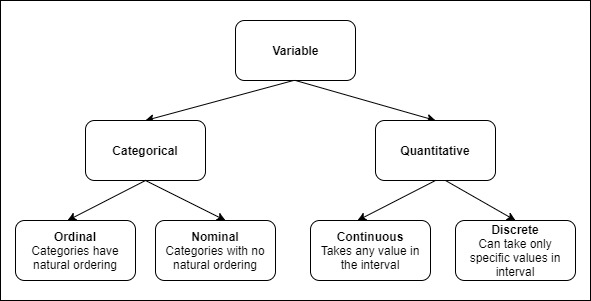
\includegraphics[scale = 0.5]{Disc1.jpg}
%chart with breakdown of categorical = ordinal or nominal, and quantitative = continuous or discrete
\end{center}

\noindent \textbf{Examples:} \\
\noindent $\bullet$ Ordinal: Education level - category of education of a student has a natural order: high school $<$ college $<$ grad. school  \\
\noindent $\bullet$ Nominal: Favorite brand of cereal \\
\noindent $\bullet$ Continuous: Height (170 cm makes sense, so does 170.5, 170.55, and 170.555) \\
\noindent $\bullet$ Discrete: Number of students in the class (can't have 16.5 students)

\noindent These distinctions are important because the kind of variable you have, determines what kind of analyses and graphs you can make.

\noindent For categorical data, only certain graphs make sense, and likewise for quantitative data.

\noindent When graphing in general, either by hand or on Minitab:
\begin{itemize}[noitemsep,nolistsep]
\item Include title, and x-axis and y-axis titles
\item Label the scale on axes
\item Include units on axes
\item Include legend/key if necessary
\end{itemize}

\noindent \textbf{Categorical Data}\\
\noindent Represented by a \textbf{bar chart}.
\begin{itemize}[noitemsep,nolistsep]
\item x-axis is the category
\item y-axis can be either frequency or relative frequency;
\noindent $relative\ frequency = \cfrac{Frequency}{Total\ Observations}$
\item Bars must have equal width
\item A Pareto diagram includes the category of "other"
\end{itemize}

\noindent \textbf{Quantitative Data} \\
\noindent Dotplot
\begin{itemize}[noitemsep, nolistsep]
\item Each dot is an observation
\item Best for sample sizes smaller than 20 - 25
\end{itemize}

\noindent Histograms \\
\noindent Stem and leaf \\
\noindent Pie charts are not good for representing quantitative data. 


\noindent \textbf{Minitab Express:} \\
\noindent You are expected to be able to generate bar chart, dotplot and draw a random sample in Minitab.

\noindent First, open Minitab Express. Load a dataset that already exists on your computer, in Minitab, click "File" $>$ "Open Worksheet"

\noindent To make a bar chart, click "Graphs" $>$ "Bar Chart".

\noindent For a dotplot, click "Graphs" $>$ "Dotplot"

\noindent Note, for quantitative variables, there's a blue curve and for categorical, there are green squares. You can't put in a categorical variable for the dot plot. 

\noindent Drawing a random sample: (1) Data $>$ Generate Patterned Data $>$ Numeric. Enter "1" to population size. (2) "Data" $>$ "Sample from Columns" and select the column you just made

 




\end{document}